\documentclass[11pt]{article}
	\usepackage[T1]{fontenc}
	\usepackage[english]{babel}
	\usepackage[utf8]{inputenc}
	\usepackage{graphicx}
	\usepackage{float}
	\usepackage{amsfonts, amsmath}
	\usepackage{fancyhdr}
	\usepackage{setspace}
	\usepackage{epstopdf}
	\usepackage{listings}
	\usepackage{color}
	\usepackage{xspace}
	\usepackage{multirow}
	\usepackage{caption}
	
	\newcommand{\latex}{\LaTeX\xspace}
	\graphicspath{images}
	
	\pagestyle{fancy}
	\fancyhead{}
	\fancyfoot{}
	\fancyfoot[R]{\thepage}
	
	\textheight 21.0cm
	\topmargin -0.5cm
	
	\setlength{\parindent}{0ex}
	\setlength{\parskip}{1em}

	\definecolor{mygreen}{rgb}{0,0.6,0}
	\definecolor{mygray}{rgb}{0.5,0.5,0.5}
	\definecolor{mymauve}{rgb}{0.58,0,0.82}

\lstset{ %
  backgroundcolor=\color{white},   % choose the background color; you must add \usepackage{color}
  basicstyle=\footnotesize,        % the size of the fonts that are used for the code
  breaklines=false,                 % sets automatic line breaking
  commentstyle=\color{mygreen},    % comment style
  frame=single,	                   % adds a frame around the code
  keepspaces=true,                 % keeps spaces in text, useful for keeping indentation of code (possibly needs columns=flexible)
  language=C++,                 % the language of the code
  numbers=left,                    % where to put the line-numbers; possible values are (none, left, right)
  numbersep=5pt,                   % how far the line-numbers are from the code
  numberstyle=\tiny\color{mygray}, % the style that is used for the line-numbers
  stepnumber=1,                    % the step between two line-numbers. If it's 1, each line will be numbered
  stringstyle=\color{mymauve},     % string literal style
  tabsize=2,	                   	 % sets default tabsize to 2 spaces
  title=\lstname                   % show the filename of files included with \lstinputlisting; also try caption instead of title
}

\renewcommand{\headrulewidth}{0pt}
			
\begin{document}
\setstretch{1.0}
\renewcommand*\contentsname{Table of contents}
	%\begin{titlepage}
	\begin{center}
		\begin{tabular}{| c | c |}
		\hline
		Wroclaw University of Technology & Dr Ewa Szlachcic\\ \hline
		Faculty of electronics & Optimization Theory and
		Numerical Methods \\
		Control Engineering and Robotics & Project - AREU0003\\
		$2^{nd}$ cycle studies & \\ \hline
		\multicolumn{2}{c}{Non-linear programming for multicriterial problems}\\
			\hline
	\end{tabular}			
	\end{center}
	
	\textbf{Topic:} Bicriterial optimization of non-linear functions with
	constraints - Niched Pareto Genetic Algorithm (NPGA).
	
	\begin{center}
		\begin{tabular}{| l | c |}
		\hline
		Authors & Tomasz Bartos, 209248\\
				& Radoslaw Zwolski, 209124\\ \hline
		Project group & Monday, 13:15-15:15, Odd weeks\\ \hline
		Project due date & 22.05.2017\\
		\hline
	\end{tabular}
	\end{center}
	
	\newpage
	
	\tableofcontents
	
	\newpage

	\section{Introduction}
	
	The aim of the project was to implement an optimization algorithm of non-linear
	bicriterial problem. Niched-Pareto Genetic Algorithm (NPGA) has been used to
	solve this problem. Whole program has been implemented in C++ using QT 	
	framework and allows user to provide functions to optimize as well 
	as configuration parameters by GUI (Graphical User Interface). An external
	library called muParser has been used to fulfill a functionality of
	function parsing .The result of algorithm has been shown as Pareto chart and
	table of non-dominated points.
	
	\section{Description of the problem and the solution}
	
	\subsection{Definition of problem}
		
	The problem is to minimize values of two functions that is provided as system
	of equations.
	
	$$\begin{cases}
		f_{1}(x_{1},x_{2},...,x_{M})\\
		f_{2}(x_{1},x_{2},...,x_{M})
	\end{cases}$$
	
	These functions can be either linear or nonlinear. Constraints given as an
	input of the algorithm are constraints of variables. So:
	
	$$\begin{cases}
		x_{1min} \leq x_{1} \leq x_{1max}\\
		x_{2min} \leq x_{2} \leq x_{2max}\\
		.\\
		.\\
		.\\
		x_{Mmin} \leq x_{M} \leq x_{Mmax}\\
	\end{cases}$$
	
	A property of such problem is that there is no way to find one optimal solution
	for both functions as usually finding the best solution in order to minimize
	one function happens to be the worst solution for minimization of the second
	function. That means that in order to solve the problem Pareto optimal points 
	have to be found as a set of points that will minimize whole system of two 
	functions. Pareto can be shown on plot axis of absenteeism being values of
	one of the functions and axis of ordinates being values of the other one.
	The idea of Pareto can be shown on Figure \ref{fig:pareto_idea} where red
	points and a line on which they lay would be optimal in Pareto sense.
	
	\begin{figure}[H]
	\caption{The idea of pareto optimal points selected from set of feasible
	points}
	\centering
	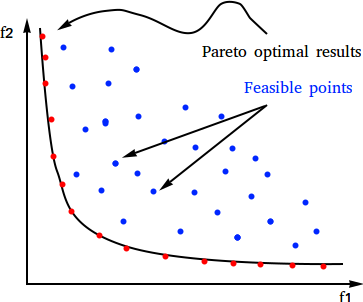
\includegraphics[scale=0.8]{pareto_definition}
	\label{fig:pareto_idea}
	\end{figure}
	
	\subsection{Description of NPGA algorithm}
	
	\begin{figure}[H]
	\caption{Flow chart presenting how the first part of NPGA works}
	\centering
	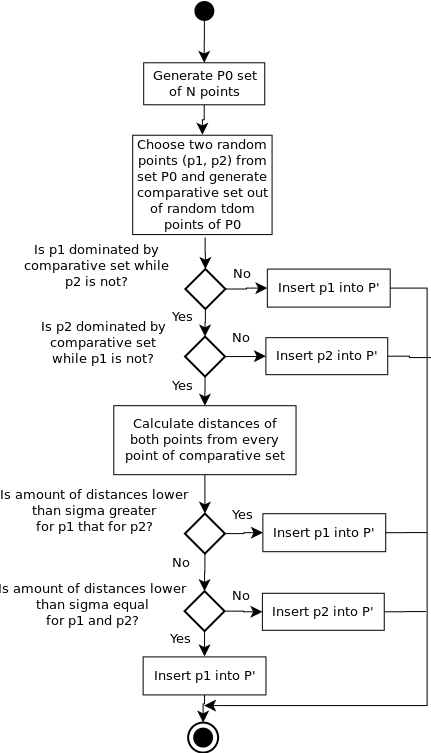
\includegraphics[scale=0.76]{NP_algorithm}
	\label{fig:NP_algorithm}
	\end{figure}
	
	To explain how does a subject point become dominated by the comparative set
	Figure \ref{fig:comparative_set} has been prepared.
	Let's say that blue points are points that are part of comparative set.
	They define a field limited by black lines that created stairs in the picture.
	When two subjects fight to become part of an optimal solution it is checked
	which one is part of these field. Figure \ref{fig:comparative_set} shows that
	for this example green point defined as one of the fighting subjects is
	part of field defined by comparative set. In resutl it becomes dominated by
	the comparative set and loses the fight. As a result red point defined as the
	other fighting subject wins the fight and joins set of non-dominated points.
	
	\begin{figure}[H]
	\caption{Defining field for which points are dominated be a comparative set}
	\centering
	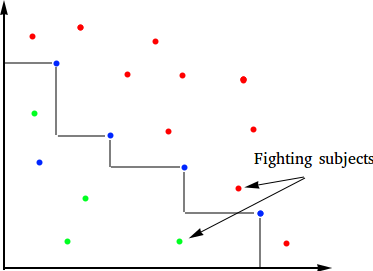
\includegraphics[scale=0.8]{comparative_set}
	\label{fig:comparative_set}
	\end{figure}
	
	There can be an occurence when none of fighting subjects wins this fight by
	being dominative to comparative set. In such case another criterion shall be
	applied. For Niched Pareto Genetic Algorithm it is checking whether a point
	satisfies niche radius criterion.
	It introduces a parameter of the algorithm called niche radius $\sigma$.
	That parameter is used to define parameter $D$ for both fighting subjects
	$pf_{1}$ and $pf_{2}$. D will be defined as:
	$$D=\sum_{i=1}^{K}\boldsymbol{1}_{<pf,p_{i}>\ <\ \sigma}$$
	So it means that $D$ is amount of points from comparative set that is closer to
	a fighting point $pf$ than $\sigma$.
	
	In the end $D$s of both fighting points are being compared and a point with
	larger $D$ parameter is being added to set of non-dominated points.
	In case of both points $D$ parameters being equal the first subject is being
	added to non-dominated set.
	
	\begin{figure}[H]
	\caption{Flow chart presenting how the second part of NPGA works
	(the part that is related to genetic evolution)}
	\centering
	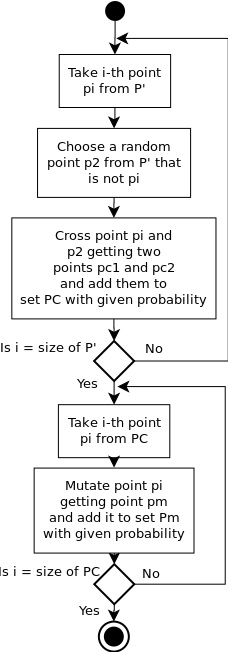
\includegraphics[scale=0.8]{GA_algorithm}
	\label{fig:GA_algorithm}
	\end{figure}
	
	Crossing over the subjects comes from theory of genetics where children inherit
	mixed traits and genes from their parents. Here traits of a subject would be
	values of particular variables and it is chosen randomly what value will a child
	inherit. For example if parent points are:
	$$(f_{1}(x), f_{2}(x)),\ x=(x_{11}, x_{21}, x_{31})$$
	$$(f_{1}(x'), f_{2}(x')),\ x'=(x_{12}, x_{22}, x_{32})$$
	
	then the children could be constructed as:
	$$(f_{1}(x''), f_{2}(x'')),\ x''=(x_{12}, x_{21}, x_{32})$$
	$$(f_{1}(x'''), f_{2}(x''')),\ x'''=(x_{11}, x_{22}, x_{31})$$
	So as it can be seen two new points have been created that have their $x_{1}$
	and $x_{3}$ values taken from one of parents and value of $x_{2}$ taken from the
	other one. That operation creates two entirely new points.
	
	The other genetic operation called mutation is about tweaking one of the gene of
	a subject, so changing a value of some randomly chosen variables a little bit to 
	create new point. For example:
	$$(f_{1}(x), f_{2}(x)),\ x=(x_{12}, x_{21}, x_{32})$$
	$$(f_{1}(x'), f_{2}(x')),\ x'=(ax_{11}, x_{22}, bx_{31})$$
	where
	$$a,\ b\in \boldsymbol{R}$$
	
	\newpage	
	\section{Application}
	
	\begin{figure}[H]
	\caption{Application window view}
	\centering
	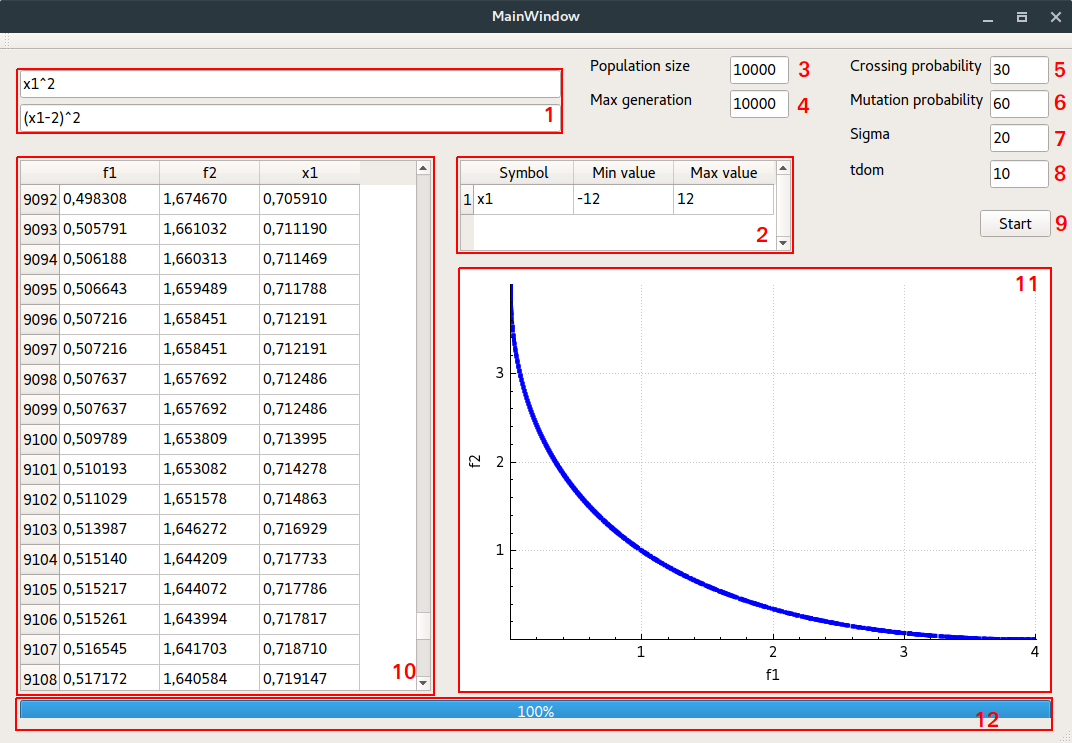
\includegraphics[scale=0.35]{application}
	\label{fig:app_window}
	\end{figure}
	
	\subsection{Interface description}	
	
	\begin{enumerate}
		\item Boxes in which user should write two functions for finding pareto
			optimal points. Top box will then be recognized as $f_{1}$ when the 
			bottom box will be recognized as $f_{2}$
		\item Table that will represent list of variables recognized in functions
			formulas that should be inserted before. Here a user can define 
			constraints of those variables writing them in "Min" and "Max" columns.
		\item Population size $N$ - amount of points that will be generated as
			($f_{1}$, $f_{2}$)
		\item Maximum generation $t$ - amount of repeats of whole algorithm
		\item Crossing probability $p_{c}$ - probability of performing crossing
			operation on a particular point.
		\item Mutation probability $p_{m}$ - probability of performing mutating
			operation on a particular point
		\item Sigma $\sigma$ - is a parameter that specifies radius of niche. It is
			distance of a chosen point 
		\item Amount of points in comparative collection $t_{dom}$
		\item Start button - clicking on it triggers start of calculations, if
			functions have been specified as well as all of parameters needed and
			described in points 1-8. If user will click on Start button before
			specifying a particular parameter it will have $0$ value by default.
		\item Table consisting points of pareto - table consisting pareto optimal
			points with value of $f_{1}$ and $f_{2}$ as well as values of every
			variable that resulted in generating such values of given functions
		\item Figure - figure showing pareto optimal points on a plot with
			coordinate system axis set as: axis of absenteeism being values of
			$f_{1}$ and axis of ordinates being values of $f_{2}$
		\item Progress bar showing progress of a testcase run to keep user in
			knowledge of progress of the calculations.
	\end{enumerate}

	\subsection{Constraints on data input}

	\begin{center}
	\captionof{table}{Fields possible to fill by a user and their acceptable 
		values}
	\begin{tabular}{| c | c | c |}
		\hline
		\textbf{Data field} & \textbf{Data type} & \textbf{Possible values}\\
		\hline
		Function & string & Attachment A\\ \hline
		Function Variables & string & x1, x2, ..., xm \\ \hline
		Min constraint & real number & $-1.7e+308 \div 1.7e+308$\\ \hline
		Max constraint & real number & $-1.7e+308 \div 1.7e+308$\\ \hline
		Population size $N$ & natural number & $0 \div 2^{31}-1$ \\ \hline
		Max generations $t$ & natural number & $0 \div 2^{31}-1$ \\ \hline
		Crossing probability & natural number & $0 \div 100$ \\ \hline
		Mutation probability & natural number & $0 \div 100$ \\ \hline
		$\sigma$ & real number & $0 \div 1.7e+308$ \\ \hline
		$t_{dom}$ & natural number & $0 \div 2^{31}-1$, $t_{dom} \leq N$ \\
		\hline
	\end{tabular}			
	\end{center}
	
	\subsection{Data validation and self-protection}
	Application contains basic mechanisms of input data validation. Following informations are verified:
	\begin{itemize}
		\item Symbol column in constrains table and cells in table with non-dominated results are write protected.
		\item Comas used in double digit representation are automatically replaced into dots.
		\item If minimal value for any symbol in constraints table is greater than maximal value, error presented on Figure \ref{fig:constraints} is shown.
		\item Application allows to write percentage values smaller than 0 and greater than 100. In both cases invalid values are interpreted respectively as 0 and 100 percent.
	\end{itemize}		
			
	\begin{figure}[H]
	\caption{Window with information about invalid constraints for \textit{x1} symbol}
	\centering
	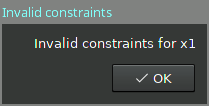
\includegraphics[scale=0.8]{constraints.png}
	\label{fig:constraints}
	\end{figure}	
	
	\newpage
	\section{Application tests}
	
	\begin{enumerate}
	
	\item Schaffer function
	$$\begin{cases}
		f_{1}(x)=x_{1}^{2}\\
		f_{2}(x)=(x_{1}-2)^{2}
	\end{cases}$$
		
	Constraints: $-A \leq x1 \leq A$, where A is $10 \leq A \leq 10^{5}$
		
	\begin{figure}[H]
	\caption{Figure of pareto optimal solutions of Schaffer function}
	\centering
	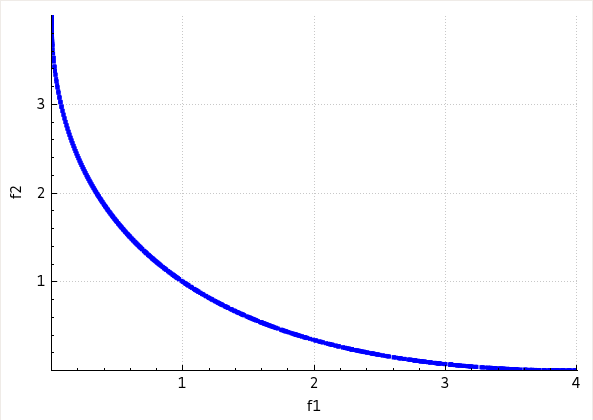
\includegraphics[scale=0.4]{schaffer}
	\label{fig:schaffer}
	\end{figure}
	
	\item Binh and Korn function
	$$\begin{cases}
		f_{1}(x)=4x_{1}^{2}+4x_{2}^{2}\\
		f_{2}(x)=(x_{1}-5)^{2}+(x_{2}-5)^{2}
	\end{cases}$$
		
	Constraints:
	$\begin{cases}
		0 \leq x_{1} \leq 3\\
		0 \leq x_{2} \leq 5
	\end{cases}$,
	
	\begin{figure}[H]
	\caption{Figure of pareto optimal solutions of Binh and Korn function}
	\centering
	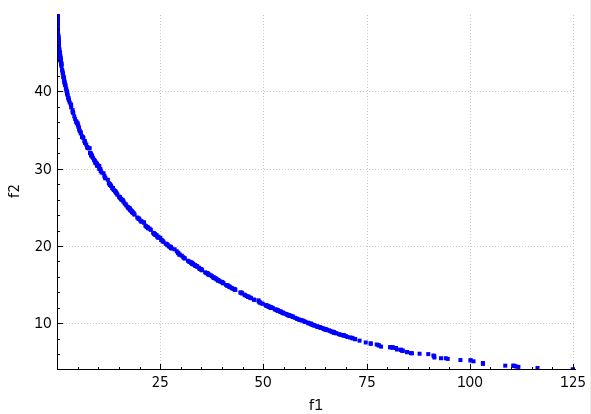
\includegraphics[scale=0.4]{binh_korn}
	\label{fig:binh_korn}
	\end{figure}
	
	\item CTP1 function (2 variables)
	$$\begin{cases}
		f_{1}(x)=x_{1}\\
		f_{2}(x)=(1+x_{2})*e^{\frac{-x_{1}}{1+x_{2}}}
	\end{cases}$$
		
	Constraints:
	$\begin{cases}
		0 \leq x_{1} \leq 1\\
		0 \leq x_{2} \leq 1
	\end{cases}$,
	
	\begin{figure}[H]
	\caption{Figure of pareto optimal solutions of Binh and Korn function}
	\centering
	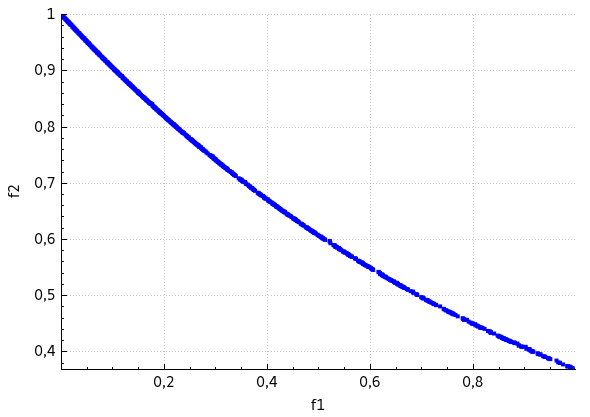
\includegraphics[scale=0.4]{ctp1}
	\label{fig:ctp1}
	\end{figure}
	
	\end{enumerate}
	
	\newpage
	\section{Conclusions}
	
	\begin{enumerate}
		\item
	\end{enumerate}
	
	\newpage	
	\section*{Attachment A}
	
	\begin{center}
	\captionof{table}{Fields possible to fill by a user and their acceptable 
		values}
	\begin{tabular}{| c | c | c |}
		\hline
		\textbf{Symbol} & \textbf{Amount of arguments} & \textbf{Function}\\ \hline
		sin & 1 & sine\\ \hline
		cos & 1 & cosine\\ \hline
		tan & 1 & tangent\\ \hline
		asin & 1 & arcsine\\ \hline
		acos & 1 & arccosine\\ \hline
		atan & 1 & arctangent\\ \hline
		sinh & 1 & hyperbolic sine\\ \hline
		cosh & 1 & hyperbolic cosine \\ \hline
		tanh & 1 & hyperbolic arctangent\\ \hline
		asinh & 1 & hyperbolic arcsine\\ \hline
		acosh & 1 & hyperbolic arccosine \\ \hline
		atanh & 1 & hyperbolic arctangent\\ \hline
		log2 & 1 & logarithm of base 2\\ \hline
		log10 & 1 & logarithm of base 10 \\ \hline
		log & 1 & logarithm of base 10\\ \hline
		ln & 1 & logarithm of base e\\ \hline
		exp & 1 & e in power of x\\ \hline
		sqrt & 1 & square root\\ \hline
		sign & 1 & signum\\ \hline
		rint & 1 & round-off to integer\\ \hline
		abs & 1 & absolute value of x\\ \hline
		min & varying & minimum of set\\ \hline
		max & varying & maximum of set\\ \hline
		sum & varying & sum of set\\ \hline
		avg & varying & mean of set\\
		\hline
	\end{tabular}			
	\end{center}
	
	\newpage	
	\begin{center}
	\captionof{table}{Fields possible to fill by a user and their acceptable 
		values}
	\begin{tabular}{| c | c | c |}
		\hline
		\textbf{Operator} & \textbf{Description} & \textbf{Priority}\\ \hline
		= & assignment & -1\\ \hline
		\&\& & logical and & -1\\ \hline
		|| & logical or & 2\\ \hline
		<= & less or equal & 4\\ \hline
		>= & greater or equal & 4\\ \hline
		!= & not equal & 4\\ \hline
		== & equal & 4\\ \hline
		< & less than & 4\\ \hline
		> & greater than & 4\\ \hline
		+ & addition & 5\\ \hline
		- & subtraction & 5\\ \hline
		* & multiplication & 6\\ \hline
		/ & division & 6\\ \hline
		\^{} & raise of x to the power of y & 7\\
		\hline
	\end{tabular}			
	\end{center}
	
	\newpage
	\section{References}
	
	\begin{enumerate}
		\item http://staff.iiar.pwr.wroc.pl/ewa.szlachcic/materialy\%
		20dydaktyczne/air\_ studia\_ 2\_ stopnia/metody\_ optymalizacji\_ wielokryterialnej\_ Mlynek.pdf
		\item MuParser main page: http://beltoforion.de/article.php?a=muparser
		\item http://beltoforion.de/article.phpa=muparser \& hl=en\& p=features\& s=idDef2\# idDef2
	\end{enumerate}
		
	
\end{document}